\chapter{Programa}\label{cap:programa}

\section{Introdução}

Este capítulo descreve o programa desenvolvido para implementar o algoritmo de
controle proposto no capítulo~\ref{cap:mapeamento}, bem como as APIs e programas
utilizados adicionalmente para possibilitar a execução de testes comparativos.

Na seção~\ref{sec:arq_prog} uma arquitetura simplificada do sistema de controle é apresentada.
Por sistema de controle, entenda-se o processo que vai desde a aquisição dos
dados da visão, planejamento e trasmissão dos comandos aos robôs.

Na seção~\ref{sec:minimax} uma implementação do algoritmo de controle conceitualizado no
capítulo~\ref{cap:mapeamento} é apresentada.

Na seção~\ref{sec:pyroboime} o programa pyroboime é descrito.

Na seção~\ref{sec:metricas} são propostas métricas para comparar o algoritmo
proposto com o utilizado anteriormente.

\section{Arquitetura do programa}\label{sec:arq_prog}

Um modelo simplificado da arquitetura do sistema de controle utilizado no para
o desenvolvimento deste projeto é apresentado na figura~\ref{fig:arq_prog}.

\begin{figure}
  \centering
  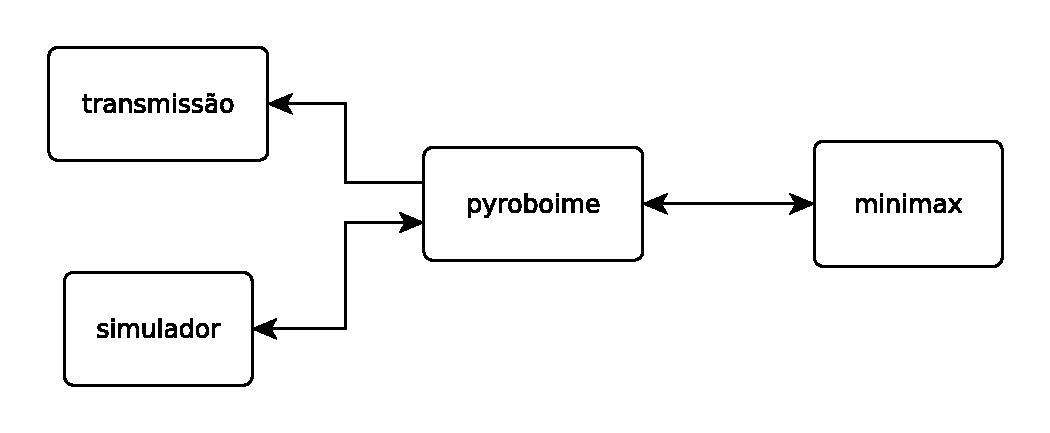
\includegraphics[width=0.8 \linewidth]{img/arq_geral_prog}
  \caption{Arquitetura simplificada do sistema de controle}\label{fig:arq_prog}
\end{figure}

\section{Processo do Minimax}\label{sec:minimax}
% disclaim: I don't think this is a good name ether...

O fluxo do programa é apresentado na figura~\ref{fig:minimax_flow}.

\begin{figure}
  \centering
  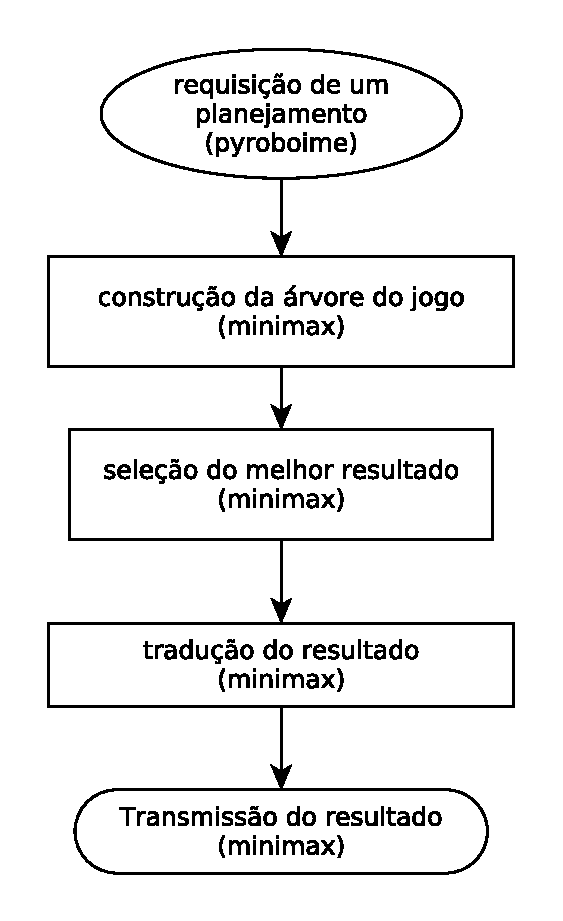
\includegraphics[width=0.2 \linewidth]{img/minimax_flow}
  \caption{Fluxo do processo minimax}\label{fig:minimax_flow}
\end{figure}

O processo de tradução consiste em transformar o planejamento obtido em uma
mensagem a ser enviada para o programa pyroboime. Para isso, foi utilizado
o protobuf. A estrutura do protocolo de resposta é apresentada no
arquivo~\ref{alg:minimax_resp_proto}. A estrutura do protocolo de atualização do
estado do tabuleiro apresentada no arquivo~\ref{alg:minimax_req_proto}.

Para otimizar os cálculos foi utilizada a API armadillo.

% Arquivo de resposta
\lstinputlisting[caption={Arquivo de definição do protocolo de resposta},
label={alg:minimax_resp_proto}]{proto/discrete.proto}

% Arquivo de requisição
\lstinputlisting[caption={Arquivo de definição do protocolo de atualização do estado do tabuleiro},
label={alg:minimax_req_proto}]{proto/update.proto}

\section{Pyroboime}\label{sec:pyroboime}
% disclaim: google translate of tdp software file

O projeto pyroboime atualmente é responsável pela inteligência artificial do
sistema de controle. Ele é baseado na arquitetura STP
(\textit{Skill-Tactic-Play}) implementada em python.
Ele é composto pelo seguintes componentes: interface com a ssl-vision,
ssl-refbox e grSim, também possui um módulo de comunicação interno para o
sistema de transmissão via rádio.

A STP é uma arquitetura de três camadas, onde o nível mais baixo, \textit{skill},
permite as manipulações de baixo nível em um único robô. A camada do meio,
\textit{tactics}, faz uso da camada de \textit{skills} para executar um nível
mais elevado de comportamento, possivelmente permitindo cooperação, mas ainda
atuando em um único robô. A camada superior, \textit{plays}, coordena as táticas
associadas a cada robô. Para maximizar o desempenho, cada \textit{play} é
implementada para se comportar de acordo com estados específicos:
\textit{stop}, \textit{halt}, \textit{indirect kicks} e jogo normal.
Uma camada de nível superior implementa como uma \textit{play} alterna entre
outras \textit{plays} baseada no estado atual do árbitro.
%Esta arquitetura é melhor representado na figura ~ \ ref {fig: stp}.
Há também uma \textit{skill} para redireccionar a partir de um joystick tal que
seja possível testar o robô com pouco esforço.

A interface é estruturada como uma pilha de filtros que liga o AI para um
conjunto flexível de \textit{updaters} (que recebe informações de estado) e
\textit{commanders} (que entregam comandos aos robôs, em ambos os ambientes simulados
e reais). Ele abstrai o ambiente externo, onde o jogo é jogado a partir da AI\@.
Entre os filtros na referida pilha, o filtro de Kalman é o responsável por
reduzir ruído vindo a partir dos dados do \textit{updater}.

O sistema de transmissão via rádio é interfaceado através da  API libusb para
controlar o hardware do transmissor, o qual está conectado via USB\@.

\section{Métricas de avaliação}\label{sec:metricas}

Atualmente o programa fornece o número soluções por segundo fornecidas pelo
algoritmo minimax. Futuramente será utilizado o algoritmo pronto para rodar
partidas simuladas contra a inteligência atual para serem levantados dados com
o objetivo de comparar de modo mais objetivo o algoritmo anterior e o
desenvolvido neste trabalho.

% vim: tw=80 et ts=2 sw=2 sts=2 ft=tex
